\begin{figure}[H]
    \centering
    \incfig{diagram0}
    \caption{Fire alarm system. Dashed components are backups.}
    \label{fig:diagram0}
\end{figure}

\hrule
\medskip

First of all, we need to determine the structure function of the system. We will separate the components of the system
hierarchically into subsystems that are either wired in parallel or in series.

% TODO: Make the descriptions aligned at the right side of the definitions  <10-05-23> 
% TODO: Make the description terms written in bold <10-05-23> 
First of all let us recognize the outer most subsystems that are wired in series:
\begin{description}[labelwidth=3cm, align=right]
    \item[\(\left\{ x_{s_1}, x_{\tilde{s_1}}, x_{s_2} \right\}\)] Smoke detectors (a.k.a. sensors) at the left side of
        diagram \ref{fig:diagram0}.

    \item[\(\left\{ x_\text{r} \right\}\)] Relay between the detectors and the fire alarms in the middle of
        diagram \ref{fig:diagram0}.

    \item[\(\left\{ x_{a_1}, x_{a_2}, x_{a_3} \right\}\)] Alarms at the entry (\(x_{a_1}\)) and the exit (\(x_{a_2}\)
        and \(x_{a_3}\)).

    \item[\(\left\{ x_\sim \right\}\)] Source of the system.
\end{description}

Starting with the sensors \(\left\{ x_{s_1}, x_{\tilde{s_1}}, x_{s_2} \right\}\), we can write the structure function of
the subsystem as a combination of two parallel structure functions. The outer parallel structure has branches \(\left\{ x_{s_2}
\right\}\) and \(\left\{ x_{s_1}, x_{\tilde{s_1}} \right\}\) where the latter is a parallel subsystem on its own with
branches \(\left\{ x_{s_1} \right\}\) and \(\left\{ x_{\tilde{s_1}} \right\}\) leading to an inner structure of
\[
    \phi\left\{ x_{s_1}, x_{\tilde{s_1}} \right\} = 1 - (1 - x_{s_1})\cdot(1- x_{\tilde{s_1}}) = \coprod_{x \in
    \{ x_{s_1}, x_{\tilde{s_1}} \}} x
\] and the outer structure function \[
\begin{split}
    \phi_s \coloneqq \phi\left\{ x_{s_1}, x_{\tilde{s_1}}, x_{s_2} \right\} &= 1 - (1 - x_{s_2}) \cdot (1 - \phi\left\{ x_{s_1},
    x_{\tilde{s_1}} \right\}) \\ 
                                                           &= 1 - (1 - x_{s_2}) \cdot (1 - (1 - (1 - x_{s_1})\cdot(1- x_{\tilde{s_1}}))) \\
                                                           &= (x_{s_2} - 1) \cdot (x_{s_1}\cdot x_{\tilde{s_1}} - x_{s_1} - x_{\tilde{s_1}}) + x_{s_2}.
\end{split}
\]

The next subsystem comprising of more than one component is the subsystem of alarms \(\left\{ x_{a_1}, x_{a_2}, x_{a_3}
\right\}\). The outer structure of this subsystem is parallel with branches \(\left\{ x_{a_1} \right\}\) and \(\left\{
x_{a_2}, x_{a_3}\right\}\). The latter (and inner) subsystem is wired in series implying the inner structure function
\[
    \phi{\left\{ x_{a_2}, x_{a_3}\right\}} = x_{a_2}\cdot x_{a_3}
\] and when combined with the outer structure, we get \[
\begin{split}
    \phi_a \coloneqq \phi {\left\{ x_{a_1}, x_{a_2}, x_{a_3} \right\}} &=  1 - (1 - x_{a_1}) \cdot (1 - \phi{\left\{ x_{a_2}, x_{a_3} \right\}}) \\
    &= 1 - (1 - x_{a_1}) \cdot (1 - x_{a_2} \cdot x_{a_3}) \\
    &= (1 - x_{a_1}) \cdot x_{a_2}\cdot x_{a_3} + x_{a_1}.
\end{split}
\]

All of the subsystems that we recognized at the beginning are wired in series so the structure function of the whole
system is
\[
    \phi(\mathbf{x}) = \phi_s \cdot x_\text{r} \cdot \phi_a \cdot x_{\sim} = \left\{ (x_{s_2} - 1) \cdot (x_{s_1}\cdot
    x_{\tilde{s_1}} - x_{s_1} - x_{\tilde{s_1}}) + x_{s_2} \right\} \cdot x_\text{r} \cdot \left\{ (1 - x_{a_1}) \cdot
x_{a_2}\cdot x_{a_3} + x_{a_1} \right\} \cdot x_{\sim}.
\] 

\begin{note*}[interpretation]
  It is important to associate the right interpretation to the calculation of reliability of the system, that we will perform
  in the next step. This depends on how we interpreted the structure function of the system based on the diagram in the
  task. 

  \begin{itemize}
    \item Since we have the sensors in the system parallel, we define the system as working if at least one of the sensor locations is
        working. That is if at least one of \(x_{s_1}\) and \(x_{\tilde{s_1}}\) or if \(x_{s_2}\) is working. That means that we
        assume that the sensors at any location are able to detect the smoke regardless of where the fire is.

    \item Similarly, we define the system as working if at least one of the alarms is working. That is, if we assume that the
        relay is switched to the alarm circuit, the alarm is ringing either at the entry or at the exit or both. 
  \end{itemize}
\end{note*}

\pagebreak

\begin{enumerate}[label = \alph*)]
    \item Determine the reliability of the system \(R(t)\) with \ac{id}~components with reliabilities \(R_i(t)\)

\begin{figure}[H]
    \centering
    \incfig{diagram1}
    \label{fig:diagram1}
    \caption{Fire alarm system. Dashed components are backups.}
\end{figure}

Where \(R_{s_1}(t) = R_{\tilde{s_1}}(t) = R_{s_2}(t) = 0.9\), \(R_{a_1}(t) = R_{a_2}(t) = R_{a_3}(t) = 0.7\), \(R_{r}(t)
= 0.8\) and \(R_\sim(t) = 0.8\).

\end{enumerate}

% \begin{figure}[H]
%     \centering
%     \resizebox{\columnwidth}{!}{
%         
\definecolor{c008000}{RGB}{0,128,0}
\definecolor{cff0000}{RGB}{255,0,0}
\definecolor{c37abc8}{RGB}{55,171,200}
\definecolor{cd35fbc}{RGB}{211,95,188}
\definecolor{cffd42a}{RGB}{255,212,42}


\def \globalscale {1.000000}
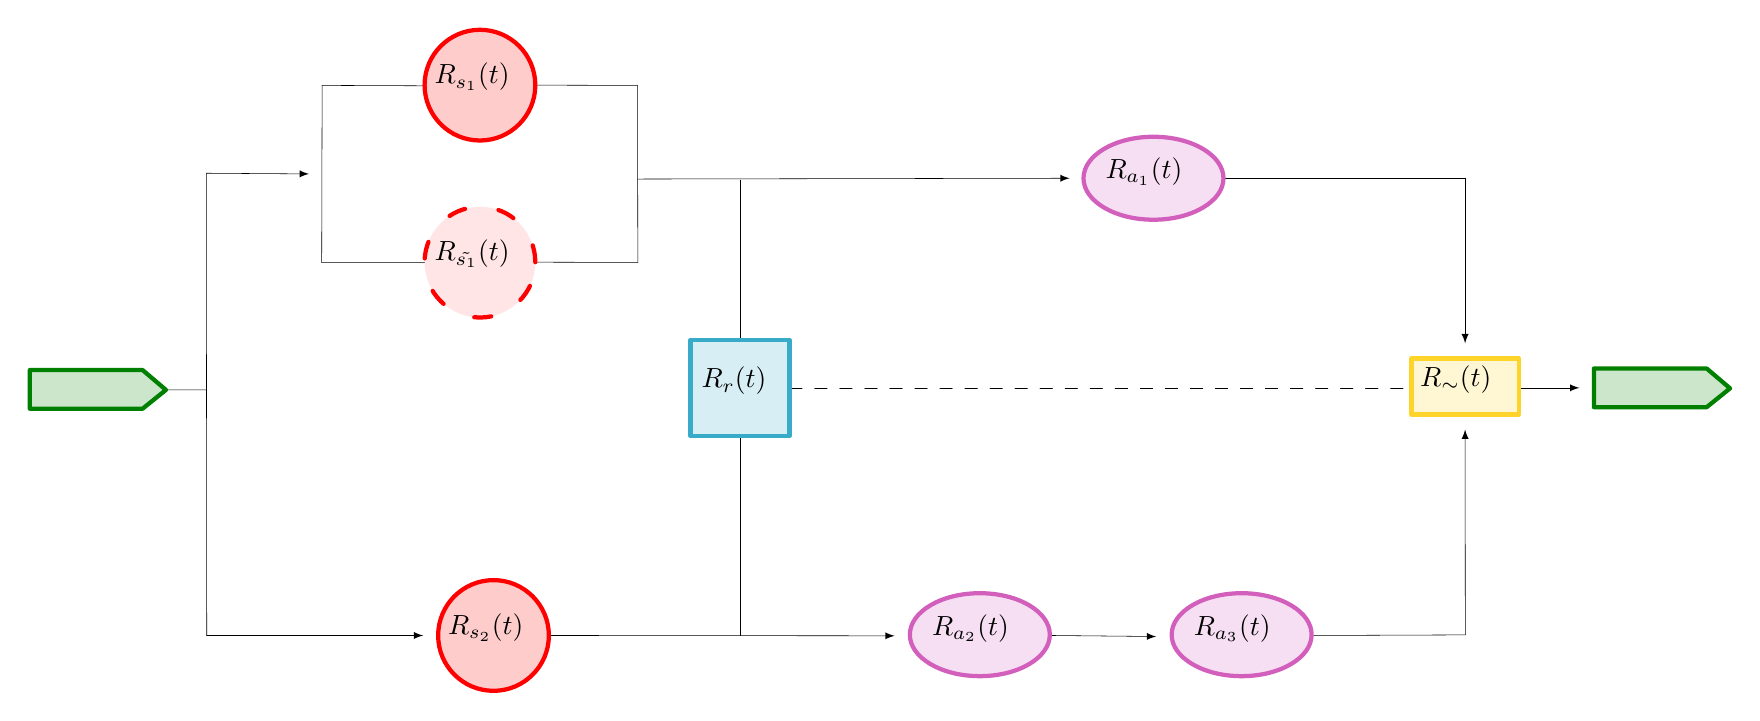
\begin{tikzpicture}[y=1cm, x=1cm, yscale=\globalscale,xscale=\globalscale, inner sep=0pt, outer sep=0pt]
\begin{scope}[shift={(0,17.700000000000003)}]
  \path[draw=black,-latex,even odd rule,line cap=round,line join=round,line
    width=0.007cm] (8.9303,-8.8752) -- (14.4163,-8.8651);



  \path[draw=black,even odd rule,line cap=round,line join=round,line
    width=0.007cm] (10.2300,-8.8885) -- (10.2300,-10.9166);



  \path[draw=black,-latex,even odd rule,line cap=round,line join=round,line
    width=0.007cm] (7.8022,-14.6719) -- (12.1938,-14.6763);



  \path[draw=black,even odd rule,line cap=round,line join=round,line
    width=0.007cm] (10.2300,-14.6719) -- (10.2300,-12.1370);



  \path[draw=black,dash pattern=on 0.159cm off 0.159cm,even odd rule,line
    cap=round,line join=round,line width=0.007cm] (10.8595,-11.5268) --
    (18.7574,-11.5268);



  \path[draw=black,-latex,even odd rule,line cap=round,line join=round,line
    width=0.007cm] (16.3697,-8.8651) -- (19.4384,-8.8651)(19.4384,-8.8651) --
    (19.4384,-10.9625);



  \path[draw=black,-latex,even odd rule,line cap=round,line join=round,line
    width=0.007cm] (14.1723,-14.6719) -- (15.5157,-14.6851);



  \path[draw=black,-latex,even odd rule,line cap=round,line join=round,line
    width=0.007cm] (19.4410,-14.6646) -- (19.4384,-12.0560);



  \path[draw=black,-latex,even odd rule,line cap=round,line join=round,line
    width=0.007cm] (20.1195,-11.5268) -- (20.8908,-11.5268);



  \path[draw=c008000,fill=c008000,fill opacity=0.200,line cap=round,line
    join=round,line width=0.054cm] (21.0742,-11.2812) -- (22.5064,-11.2812) --
    (22.8032,-11.5334) -- (22.5064,-11.7725) -- (21.0742,-11.7725) -- cycle;



  \path[draw=black,even odd rule,line cap=round,line join=round,line
    width=0.007cm] (17.5163,-14.6719) -- (19.4410,-14.6646);



  \path[draw=black,even odd rule,line cap=round,line join=round,line
    width=0.007cm] (8.9285,-7.6860) -- (8.9321,-9.9343);



  \path[draw=black,even odd rule,line cap=round,line join=round,line
    width=0.007cm] (7.6301,-7.6828) -- (8.9285,-7.6860);



  \path[draw=black,even odd rule,line cap=round,line join=round,line
    width=0.007cm] (7.6301,-9.9311) -- (8.9321,-9.9343);



  \path[draw=black,even odd rule,line cap=round,line join=round,line
    width=0.007cm] (4.9227,-7.6860) -- (6.2186,-7.6912);



  \path[draw=black,even odd rule,line cap=round,line join=round,line
    width=0.007cm] (4.9173,-9.9343) -- (6.2241,-9.9335);



  \path[draw=black,even odd rule,line cap=round,line join=round,line
    width=0.007cm] (4.9227,-7.6860) -- (4.9173,-9.9343);



  \path[draw=black,even odd rule,line cap=round,line join=round,line
    width=0.007cm] (3.4542,-11.5334) -- (3.4525,-8.8016);



  \path[draw=black,-latex,even odd rule,line cap=round,line join=round,line
    width=0.007cm] (3.4525,-8.8016) -- (4.7570,-8.8102);



  \path[draw=black,even odd rule,line cap=round,line join=round,line
    width=0.007cm] (3.4542,-11.5334) -- (3.4574,-14.6719);



  \path[draw=black,-latex,even odd rule,line cap=round,line join=round,line
    width=0.007cm] (3.4574,-14.6719) -- (6.2062,-14.6719);



  \path[draw=cff0000,fill=cff0000,dash pattern=on 0.216cm off 0.432cm,fill
    opacity=0.100,line cap=round,line join=round,line width=0.054cm] (6.9271,
    -9.9311) circle (0.7030cm);



  \path[draw=c37abc8,fill=c37abc8,fill opacity=0.200,line cap=round,line
    join=round,line width=0.054cm,rounded corners=0.0000cm] (9.6005211,
    -10.916614000000003) rectangle (10.8595039, -12.137025400000002);



  \path[draw=cd35fbc,fill=cd35fbc,fill opacity=0.200,line cap=round,line
    join=round,line width=0.054cm] (15.4809, -8.8651) ellipse (0.8888cm and
    0.5268cm);



  \path[draw=cffd42a,fill=cffd42a,fill opacity=0.200,line cap=round,line
    join=round,line width=0.054cm,rounded corners=0.0000cm] (18.757355,
    -11.153033) rectangle (20.1194643, -11.86532915);



  \path[draw=cff0000,fill=cff0000,fill opacity=0.200,line cap=round,line
    join=round,line width=0.054cm] (6.9271, -7.6828) circle (0.7030cm);



  \path[draw=cd35fbc,fill=cd35fbc,fill opacity=0.200,line cap=round,line
    join=round,line width=0.054cm] (13.2755, -14.6618) ellipse (0.8888cm and
    0.5268cm);



  \path[draw=cd35fbc,fill=cd35fbc,fill opacity=0.200,line cap=round,line
    join=round,line width=0.054cm] (16.6004, -14.6618) ellipse (0.8888cm and
    0.5268cm);



  \path[draw=cff0000,fill=cff0000,fill opacity=0.200,line cap=round,line
    join=round,line width=0.054cm] (7.0992, -14.6719) circle (0.7030cm);



  \path[fill=black,line width=0.026cm] (14.8742,-8.9578) node[above right]
    (text1681){$R_{a_1}(t)$};



  \path[fill=black,line width=0.026cm] (6.3506,-10.0037) node[above right]
    (text1153){$R_{\tilde{s_1}}(t)$};



  \path[fill=black,line width=0.026cm] (9.7427,-11.6164) node[above right]
    (text1669){$R_\text{r}(t)$};



  \path[fill=black,line width=0.026cm] (18.8688,-11.5976) node[above right]
    (text371){$R_\sim(t)$};



  \path[fill=black,line width=0.026cm] (6.3506,-7.7553) node[above right]
    (text1249){$R_{s_1}(t)$};



  \path[fill=black,line width=0.026cm] (12.6688,-14.7544) node[above right]
    (text1610){$R_{a_2}(t)$};



  \path[fill=black,line width=0.026cm] (15.9937,-14.7544) node[above right]
    (text1668){$R_{a_3}(t)$};



  \path[fill=black,line width=0.026cm] (6.5227,-14.7444) node[above right]
    (text1722){$R_{s_2}(t)$};



  \path[draw=black,even odd rule,line cap=butt,line join=miter,line width=0.007cm]
    (2.9392,-11.5533) -- (3.4543,-11.5531);



  \path[draw=black,even odd rule,line cap=butt,line join=miter,line width=0.007cm]
    (3.4410,-11.6115) -- (3.4410,-11.6115);



  \path[draw=c008000,fill=c008000,fill opacity=0.200,line cap=round,line
    join=round,line width=0.054cm] (1.2102,-11.3010) -- (2.6423,-11.3010) --
    (2.9392,-11.5533) -- (2.6423,-11.7923) -- (1.2102,-11.7923) -- cycle;



\end{scope}

\end{tikzpicture}

%     }
%     \caption{Fire alarm system. Dashed components are backups.}
% \end{figure}

\hrule
\medskip

Since we have already determined the structural function of the system \(\phi(\mathbf{x})\), and we have
\ac{id}~components, this will be very easy.
\[
    \begin{split}
        R(t) &= \mathbb{E}\left[\phi(\mathbf{X}(t)) \right] = \mathbb{E}\left[\left\{ (X_{s_2} - 1) \cdot (X_{s_1}\cdot
    X_{\tilde{s_1}} - X_{s_1} - X_{\tilde{s_1}}) + X_{s_2} \right\} \cdot X_\text{r} \cdot \left\{ (1 - X_{a_1}) \cdot
X_{a_2}\cdot X_{a_3} + X_{a_1} \right\} \cdot X_{\sim}  \right] \\
             &\overset{\text{\ac{id}}}{=} \left\{ (R_{s_2}(t) - 1) \cdot (R_{s_1}(t)\cdot
    R_{\tilde{s_1}}(t) - R_{s_1}(t) - R_{\tilde{s_1}})(t) + R_{s_2}(t) \right\} \cdot R_\text{r}(t) \cdot \left\{ (1
    - R_{a_1}(t)) \cdot
R_{a_2}(t)\cdot R_{a_3}(t) + R_{a_1}(t) \right\} \cdot R_{\sim}(t).
    \end{split}
\] 

The last step we need to finish is to substitute the values from the task. And since the reliabilities are constant in
time we have a constant reliability

\begin{equation*}
      R(t) = R = 0.54153792.
\end{equation*}
    
\pagebreak

\begin{enumerate}[label = \alph*), resume]
    \item Find the \ac{MTTF} of the system of \ac{iid}~components with constant failure rates \(r_i(t) = \lambda \)

\begin{figure}[H]
    \centering
    \incfig{diagram2}
    \label{fig:diagram2}
    \caption{Fire alarm system. Dashed components are backups.}
\end{figure}

Where \(r_{s_1}(t) = r_{\tilde{s_1}}(t) = r_{s_2}(t) = r_{a_1}(t) = r_{a_2}(t) = r_{a_3}(t) = r_{r}(t)
= r_\sim(t) = \lambda\).

\end{enumerate}

\hrule
\medskip

% \begin{figure}[H]
%     \centering
%     \resizebox{\columnwidth}{!}{
%         
\definecolor{c008000}{RGB}{0,128,0}
\definecolor{cff0000}{RGB}{255,0,0}
\definecolor{c37abc8}{RGB}{55,171,200}
\definecolor{cd35fbc}{RGB}{211,95,188}
\definecolor{cffd42a}{RGB}{255,212,42}


\def \globalscale {1.000000}
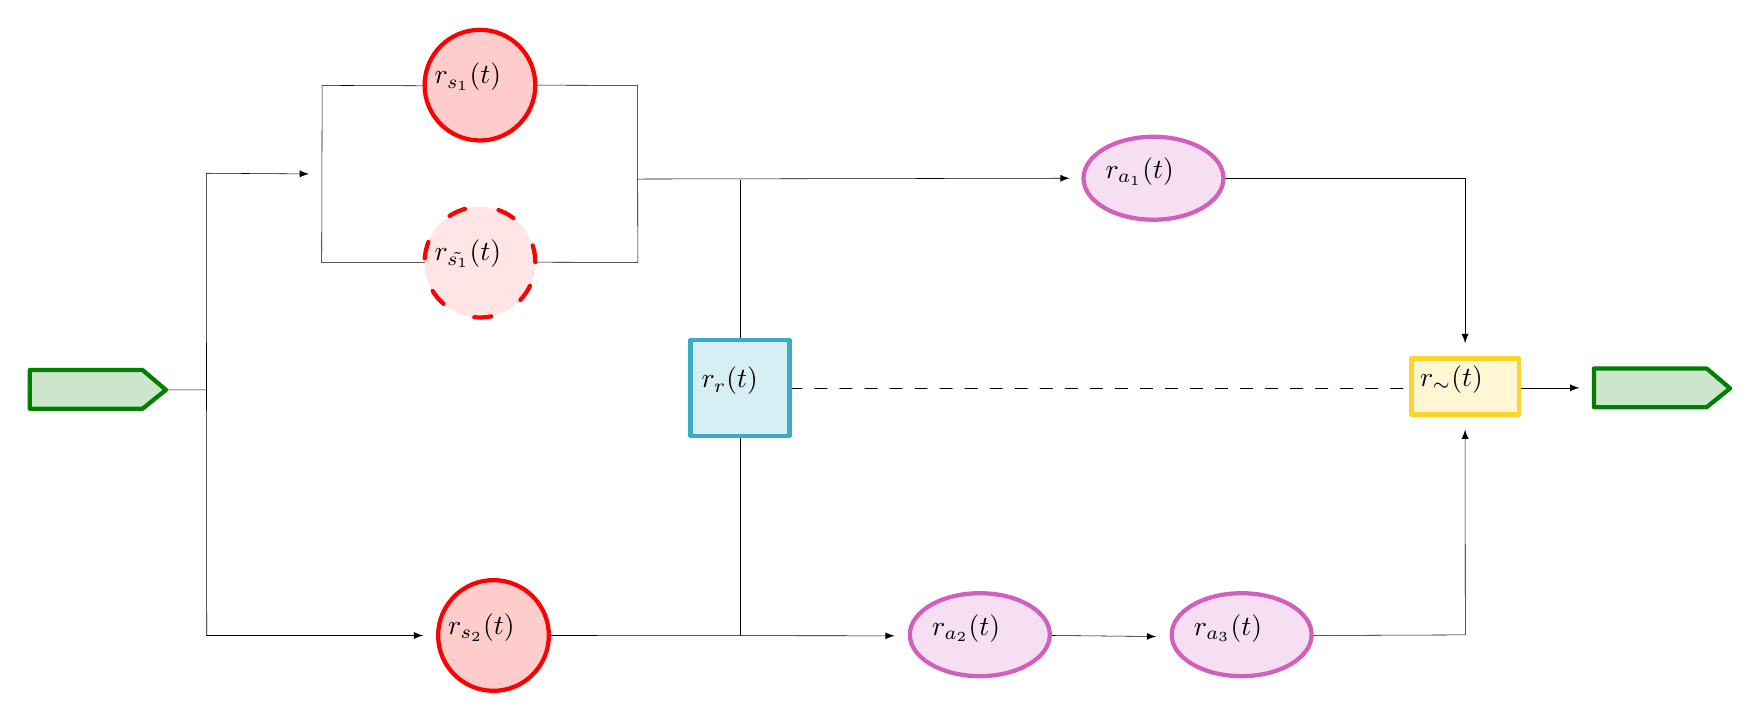
\begin{tikzpicture}[y=1cm, x=1cm, yscale=\globalscale,xscale=\globalscale, inner sep=0pt, outer sep=0pt]
\begin{scope}[shift={(0,17.700000000000003)}]
  \path[draw=black,-latex,even odd rule,line cap=round,line join=round,line
    width=0.007cm] (8.8770,-9.3012) -- (14.3630,-9.2911);



  \path[draw=black,even odd rule,line cap=round,line join=round,line
    width=0.007cm] (10.1767,-9.3145) -- (10.1767,-11.3426);



  \path[draw=black,-latex,even odd rule,line cap=round,line join=round,line
    width=0.007cm] (7.7489,-15.0979) -- (12.1406,-15.1023);



  \path[draw=black,even odd rule,line cap=round,line join=round,line
    width=0.007cm] (10.1767,-15.0979) -- (10.1767,-12.5630);



  \path[draw=black,dash pattern=on 0.159cm off 0.159cm,even odd rule,line
    cap=round,line join=round,line width=0.007cm] (10.8062,-11.9528) --
    (18.7041,-11.9528);



  \path[draw=black,-latex,even odd rule,line cap=round,line join=round,line
    width=0.007cm] (16.3164,-9.2911) -- (19.3851,-9.2911)(19.3851,-9.2911) --
    (19.3851,-11.3885);



  \path[draw=black,-latex,even odd rule,line cap=round,line join=round,line
    width=0.007cm] (14.1190,-15.0979) -- (15.4625,-15.1111);



  \path[draw=black,-latex,even odd rule,line cap=round,line join=round,line
    width=0.007cm] (19.3877,-15.0906) -- (19.3851,-12.4820);



  \path[draw=black,-latex,even odd rule,line cap=round,line join=round,line
    width=0.007cm] (20.0662,-11.9528) -- (20.8375,-11.9528);



  \path[draw=c008000,fill=c008000,fill opacity=0.200,line cap=round,line
    join=round,line width=0.054cm] (21.0210,-11.7072) -- (22.4531,-11.7072) --
    (22.7500,-11.9594) -- (22.4531,-12.1985) -- (21.0210,-12.1985) -- cycle;



  \path[draw=black,even odd rule,line cap=round,line join=round,line
    width=0.007cm] (17.4630,-15.0979) -- (19.3877,-15.0906);



  \path[draw=black,even odd rule,line cap=round,line join=round,line
    width=0.007cm] (8.8753,-8.1120) -- (8.8788,-10.3603);



  \path[draw=black,even odd rule,line cap=round,line join=round,line
    width=0.007cm] (7.5768,-8.1088) -- (8.8753,-8.1120);



  \path[draw=black,even odd rule,line cap=round,line join=round,line
    width=0.007cm] (7.5768,-10.3571) -- (8.8788,-10.3603);



  \path[draw=black,even odd rule,line cap=round,line join=round,line
    width=0.007cm] (4.8695,-8.1120) -- (6.1653,-8.1172);



  \path[draw=black,even odd rule,line cap=round,line join=round,line
    width=0.007cm] (4.8640,-10.3603) -- (6.1709,-10.3595);



  \path[draw=black,even odd rule,line cap=round,line join=round,line
    width=0.007cm] (4.8695,-8.1120) -- (4.8640,-10.3603);



  \path[draw=black,even odd rule,line cap=round,line join=round,line
    width=0.007cm] (3.4010,-11.9594) -- (3.3992,-9.2276);



  \path[draw=black,-latex,even odd rule,line cap=round,line join=round,line
    width=0.007cm] (3.3992,-9.2276) -- (4.7038,-9.2362);



  \path[draw=black,even odd rule,line cap=round,line join=round,line
    width=0.007cm] (3.4010,-11.9594) -- (3.4041,-15.0979);



  \path[draw=black,-latex,even odd rule,line cap=round,line join=round,line
    width=0.007cm] (3.4041,-15.0979) -- (6.1529,-15.0979);



  \path[draw=cff0000,fill=cff0000,dash pattern=on 0.216cm off 0.432cm,fill
    opacity=0.100,line cap=round,line join=round,line width=0.054cm] (6.8738,
    -10.3571) circle (0.7030cm);



  \path[draw=c37abc8,fill=c37abc8,fill opacity=0.200,line cap=round,line
    join=round,line width=0.054cm,rounded corners=0.0000cm] (9.547254200000001,
    -11.342616) rectangle (10.806237000000001, -12.5630274);



  \path[draw=cd35fbc,fill=cd35fbc,fill opacity=0.200,line cap=round,line
    join=round,line width=0.054cm] (15.4276, -9.2911) ellipse (0.8888cm and
    0.5268cm);



  \path[draw=cffd42a,fill=cffd42a,fill opacity=0.200,line cap=round,line
    join=round,line width=0.054cm,rounded corners=0.0000cm] (18.704088000000002,
    -11.579036000000002) rectangle (20.066197300000002, -12.291332150000002);



  \path[draw=cff0000,fill=cff0000,fill opacity=0.200,line cap=round,line
    join=round,line width=0.054cm] (6.8738, -8.1088) circle (0.7030cm);



  \path[draw=cd35fbc,fill=cd35fbc,fill opacity=0.200,line cap=round,line
    join=round,line width=0.054cm] (13.2223, -15.0878) ellipse (0.8888cm and
    0.5268cm);



  \path[draw=cd35fbc,fill=cd35fbc,fill opacity=0.200,line cap=round,line
    join=round,line width=0.054cm] (16.5471, -15.0878) ellipse (0.8888cm and
    0.5268cm);



  \path[draw=cff0000,fill=cff0000,fill opacity=0.200,line cap=round,line
    join=round,line width=0.054cm] (7.0459, -15.0979) circle (0.7030cm);



  \path[fill=black,line width=0.026cm] (14.8209,-9.3838) node[above right]
    (text1681){$r_{a_1}(t)$};



  \path[fill=black,line width=0.026cm] (6.2973,-10.4297) node[above right]
    (text1153){$r_{\tilde{s_1}}(t)$};



  \path[fill=black,line width=0.026cm] (9.6894,-12.0424) node[above right]
    (text1669){$r_\text{r}(t)$};



  \path[fill=black,line width=0.026cm] (18.8156,-12.0236) node[above right]
    (text371){$r_\sim(t)$};



  \path[fill=black,line width=0.026cm] (6.2973,-8.1813) node[above right]
    (text1249){$r_{s_1}(t)$};



  \path[fill=black,line width=0.026cm] (12.6156,-15.1804) node[above right]
    (text1610){$r_{a_2}(t)$};



  \path[fill=black,line width=0.026cm] (15.9405,-15.1804) node[above right]
    (text1668){$r_{a_3}(t)$};



  \path[fill=black,line width=0.026cm] (6.4694,-15.1704) node[above right]
    (text1722){$r_{s_2}(t)$};



  \path[draw=black,even odd rule,line cap=butt,line join=miter,line width=0.007cm]
    (2.8859,-11.9793) -- (3.4010,-11.9791);



  \path[draw=black,even odd rule,line cap=butt,line join=miter,line width=0.007cm]
    (3.3877,-12.0375) -- (3.3877,-12.0375);



  \path[draw=c008000,fill=c008000,fill opacity=0.200,line cap=round,line
    join=round,line width=0.054cm] (1.1569,-11.7270) -- (2.5891,-11.7270) --
    (2.8859,-11.9793) -- (2.5891,-12.2183) -- (1.1569,-12.2183) -- cycle;



\end{scope}

\end{tikzpicture}

%     }
%     \caption{Fire alarm system. Dashed components are backups.}
% \end{figure}
